\documentclass[10pt]{article}
\usepackage[margin=0.72in]{geometry}
\setlength{\columnsep}{0.24in}
\usepackage{times}
\usepackage{graphicx}
\usepackage{pgfplots}
\pgfplotsset{compat=1.18}
\usepackage{booktabs}
\usepackage{amsmath,amssymb}
\usepackage{microtype}
\usepackage{url}
\usepackage{natbib}
\usepackage[colorlinks=true,allcolors=blue]{hyperref}
\usepackage{enumitem}
\usepackage{caption}
\usepackage{float}
\usepackage{needspace}
\usepackage{flushend}
\captionsetup{font=small,labelfont=bf}
\setlist[itemize]{leftmargin=1.25em,itemsep=1.5pt,topsep=3pt}
\flushbottom
\emergencystretch=1.2em
\tolerance=1200
\pretolerance=700
\widowpenalties 3 10000 10000 0
\clubpenalties 3 10000 10000 0
\displaywidowpenalty=10000
\hypersetup{
  pdfauthor={Victor Lavrenko},
  pdftitle={The Gogol Effect in LLMs: Post-Completion Self-Devaluation},
  pdfsubject={Post-completion self-devaluation and state-dependent self-evaluation in large language models},
  pdfkeywords={large language models, self-evaluation, Gogol effect, post-completion self-devaluation, IKEA effect, self-attribution bias, ownership bias, confidence}
}

\title{\textbf{The Gogol Effect in LLMs:}\\[2pt]\large Post-Completion Self-Devaluation}
\author{Victor Lavrenko\\PeaceTech VC, Israel\\\texttt{victor@peacetech.vc}}
\date{23 September 2026}

\newcommand{\live}{\textsc{Live}}
\newcommand{\replay}{\textsc{Replay}}
\newcommand{\post}{\textsc{Post}}
\newcommand{\papersection}[1]{\Needspace{4.4\baselineskip}\section{#1}}
\newcommand{\papersubsection}[1]{\Needspace{3.8\baselineskip}\subsection{#1}}
% Vector figure definitions. Both are drawn directly by TikZ/PGFPlots.
\pgfplotsset{
  paperplot/.style={
    tick label style={font=\scriptsize},
    label style={font=\scriptsize},
    grid style={black!10},
    axis line style={black!75},
    tick style={black!75},
    clip=false,
  }
}

\newcommand{\SixModelEffectsPlot}{%
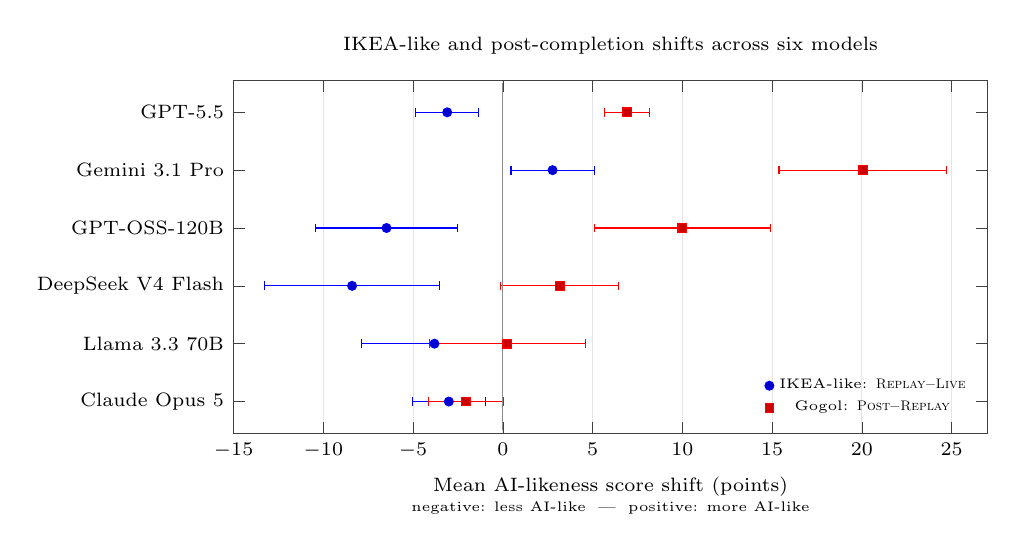
\begin{tikzpicture}[font=\scriptsize]
\begin{axis}[
  width=.92\linewidth,
  height=.50\linewidth,
  xmin=-15, xmax=27,
  xtick={-15,-10,-5,0,5,10,15,20,25},
  ymin=-0.55, ymax=5.55,
  y dir=reverse,
  ytick={0,1,2,3,4,5},
  yticklabels={GPT-5.5,Gemini 3.1 Pro,GPT-OSS-120B,DeepSeek V4 Flash,Llama 3.3 70B,Claude Opus 5},
  paperplot,
  title style={font=\scriptsize},
  title={IKEA-like and post-completion shifts across six models},
  xlabel={\shortstack{Mean AI-likeness score shift (points)\\[-1pt]\tiny negative: less AI-like \;|\; positive: more AI-like}},
  xmajorgrids,
  legend style={
    at={(0.99,0.02)}, anchor=south east,
    draw=none, fill=none,
    font=\tiny,
    row sep=-1pt,
  },
]
\addplot+[
  only marks, mark=*, mark size=1.6pt,
  error bars/.cd, x dir=both, x explicit,
] table[x=x,y=y,x error minus=em,x error plus=ep,row sep=\\]{
 x      y   em      ep\\
-3.10   0   1.766   1.763\\
 2.77   1   2.316   2.319\\
-6.48   2   3.967   3.974\\
-8.40   3   4.861   4.861\\
-3.81   4   4.077   4.075\\
-3.01   5   2.031   2.027\\
};
\addlegendentry{IKEA-like: \replay{}--\live{}}
\addplot+[
  only marks, mark=square*, mark size=1.55pt,
  error bars/.cd, x dir=both, x explicit,
] table[x=x,y=y,x error minus=em,x error plus=ep,row sep=\\]{
 x      y   em      ep\\
 6.91   0   1.267   1.272\\
20.06   1   4.673   4.663\\
10.00   2   4.905   4.900\\
 3.18   3   3.288   3.278\\
 0.24   4   4.343   4.342\\
-2.05   5   2.100   2.106\\
};
\addlegendentry{Gogol: \post{}--\replay{}}
\draw[black!45,thin] (axis cs:0,-.5) -- (axis cs:0,5.5);
\end{axis}
\end{tikzpicture}
}

\newcommand{\ReliabilityMapPlot}{%
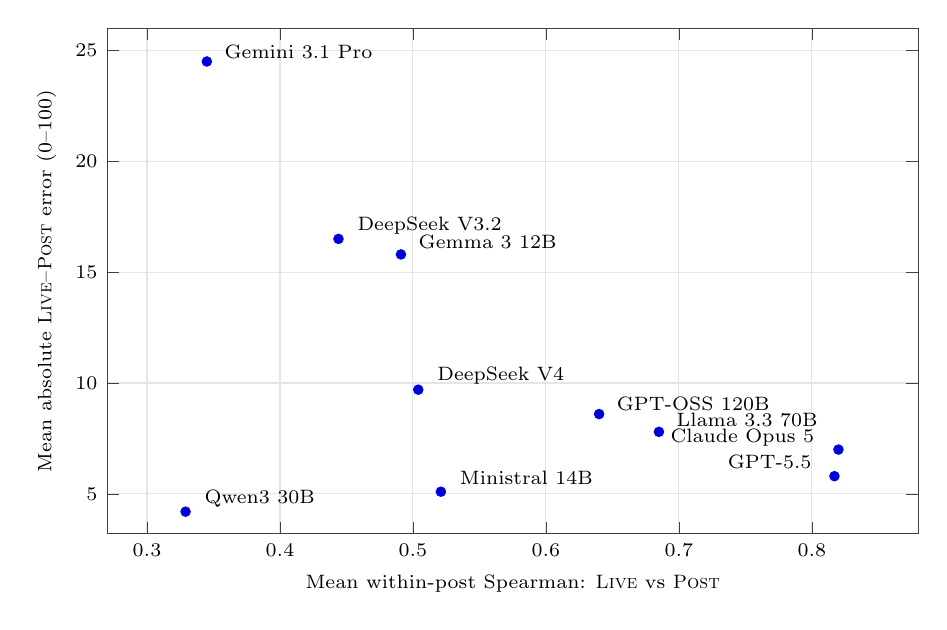
\begin{tikzpicture}[font=\scriptsize]
\begin{axis}[
  width=.98\linewidth,
  height=.66\linewidth,
  xmin=.27, xmax=.88,
  ymin=3.2, ymax=26.0,
  xtick={.3,.4,.5,.6,.7,.8},
  ytick={5,10,15,20,25},
  xlabel={Mean within-post Spearman: \live{} vs \post{}},
  ylabel={Mean absolute \live{}--\post{} error (0--100)},
  paperplot,
  xmajorgrids, ymajorgrids,
]
\addplot+[only marks, mark=*, mark size=1.7pt] coordinates {
  (.820,7.0) (.817,5.8) (.685,7.8) (.640,8.6) (.521,5.1)
  (.504,9.7) (.491,15.8) (.444,16.5) (.345,24.5) (.329,4.2)
};
\node[anchor=west] at (axis cs:.351,24.95) {Gemini 3.1 Pro};
\node[anchor=west] at (axis cs:.451,17.10) {DeepSeek V3.2};
\node[anchor=west] at (axis cs:.497,16.38) {Gemma 3 12B};
\node[anchor=west] at (axis cs:.511,10.35) {DeepSeek V4};
\node[anchor=west] at (axis cs:.646,9.05) {GPT-OSS 120B};
\node[anchor=west] at (axis cs:.691,8.35) {Llama 3.3 70B};
\node[anchor=east] at (axis cs:.809,7.55) {Claude Opus 5};
\node[anchor=east] at (axis cs:.807,6.45) {GPT-5.5};
\node[anchor=west] at (axis cs:.528,5.75) {Ministral 14B};
\node[anchor=west] at (axis cs:.336,4.80) {Qwen3 30B};
\end{axis}
\end{tikzpicture}
}


\begin{document}
\twocolumn[
\begin{@twocolumnfalse}
\maketitle
\vspace{-1.7em}
\end{@twocolumnfalse}
]
\begin{abstract}
Prior work shows that LLMs can favor content attributed to themselves, suggesting an IKEA-like self-bias. We test whether this explains why models evaluate their own text differently during generation and after completion. A \live{}--\replay{}--\post{} protocol separates an IKEA-like writer-state shift (\replay{}--\live{}) from post-completion self-devaluation (\post{}--\replay{}). Across six models with \live{}--\replay{}--\post{} data, only one has a positive mean IKEA-like shift ($+2.8$ points); the other five shift in the opposite direction. By contrast, four of six show positive evidence of post-completion self-devaluation, with mean shifts from $+3.2$ to $+20.1$ points; the remaining two are near zero ($+0.2$) or negative ($-2.0$). In the strongest case, 88\% of the total \live{}--\post{} change emerges only after completion. We call this model-dependent pattern the \emph{Gogol effect}: a model judges its own earlier text more harshly once it can inspect the finished output.
\end{abstract}
\vspace{0.4em}

\papersection{Introduction}
Large language models increasingly evaluate their own intermediate outputs. Agents critique actions before execution, reasoning systems score partial trajectories, and iterative generation methods use self-evaluation to decide whether to continue, revise, or abandon an answer. Yet the score produced \emph{during} generation is not necessarily the score the same model would assign after the output is complete.

One plausible explanation is an LLM analogue of the human \emph{IKEA effect}, in which people can value products more after contributing labor to them \citep{norton2012ikea}. Recent LLM work makes that analogy plausible: models can favor outputs associated with themselves or their model family, exhibit self-attribution bias when an action is implicitly framed as their own, and report greater confidence in identical answers when those answers appear as their own assistant response \citep{panickssery2024recognize,xu2024pride,khullar2026selfattribution,sanzguerrero2026ownership}. If this is what drives \live{}-versus-retrospective disagreement, then a model should become less favorable to the same partial output when moved from the original writing trajectory into a fresh observer-like evaluation.

But there is another possibility. A sentence that looked acceptable when written may look repetitive, formulaic, inconsistent, or otherwise weak once the entire response is visible. In that case, the main shift should occur not when the model leaves the writing trajectory, but only after the completed work can be inspected as a whole. We call this second pattern \emph{post-completion self-devaluation}. For memorability, we refer to it as the \emph{Gogol effect}: Nikolai Gogol, a Russian writer of Ukrainian origin, labored for years on the second part of \emph{Dead Souls} and famously burned most of the manuscript shortly before his death \citep{gogolbio}. The name is a literary metaphor, not a claim that language models experience regret, ownership, or any human mental state.

We distinguish the two patterns with a three-state protocol. \live{} records the score emitted on the original generation trajectory. \replay{} reconstructs the visible prefix through the same sentence in a fresh call. \post{} asks for a retrospective score after the complete output is visible. For sentence $i$ in output $q$, let the corresponding scores be $L_{qi}$, $R_{qi}$, and $P_{qi}$. Then
\begin{equation}
P-L=(R-L)+(P-R).
\label{eq:decomp}
\end{equation}
The identity is exact, although its causal interpretation is not. On our scale, higher scores mean ``more likely to appear AI-generated,'' so a positive $R-L$ means that \live{} was more favorable than \replay{} and is therefore directionally consistent with an IKEA-like writer/self-attribution effect. A positive $P-R$ means that the model judges the earlier text more harshly after seeing the completed output; this is the operational signature we call the Gogol effect.

Our probe asks models to generate short social-network posts and, after each sentence, score from 0 to 100 how likely an average reader would be to regard that sentence as AI-generated. The endpoint is intentionally easy to elicit both online and retrospectively, but it is not a validated probability of human detection and it is not factual-confidence calibration. The experiment therefore studies \emph{state dependence in self-evaluation}, not general correctness overconfidence.

The central empirical result becomes clearer when \replay{} is available across model families. Among six models with \live{}--\replay{}--\post{} data, only Gemini has a positive mean \replay{}--\live{} shift ($+2.77$ points); the other five means are negative, ranging from $-3.01$ to $-8.40$. \post{}--\replay{} behaves differently. GPT-5.5, Gemini~3.1 Pro, GPT-OSS-120B, and DeepSeek~V4 Flash show positive post-completion shifts of $+6.91$, $+20.06$, $+10.00$, and $+3.18$ points, respectively, whereas Llama~3.3 70B is near zero ($+0.24$) and Claude Opus~5 trends in the opposite direction ($-2.05$). Thus IKEA-like self-favoring is uncommon and modest in this sample, while the Gogol effect appears in more models and can be substantially larger. The effect is nevertheless model-dependent rather than universal.

\paragraph{Contributions.}
\begin{itemize}
    \item We distinguish two phenomena that a simple \live{}--\post{} comparison conflates: an IKEA-like writer/self-attribution component ($R-L$) and post-completion self-devaluation ($P-R$), which we call the Gogol effect.
    \item We introduce a matched \live{}--\replay{}--\post{} protocol that operationally decomposes the retrospective shift while making explicit the limits of hosted-model \replay{} as a causal intervention.
    \item Across six decomposed models, only one has a positive mean IKEA-like shift, whereas four show positive evidence of a Gogol effect. Among those four, mean \post{}--\replay{} shifts range from $+3.18$ to $+20.06$ points; two additional models show no positive effect at the available sample sizes.
    \item A cost-controlled adaptive \replay{} extension broadens the decomposition beyond the two original confirmation models. Fresh-extension sequential tests support the positive Gogol effect in GPT-OSS-120B and DeepSeek~V4 Flash, while Claude Opus~5 and Llama~3.3 70B remain negative or near zero through 24 prompts.
    \item We show that score-level shifts and within-output ranking stability are separable, which matters for systems that use self-scores to choose which span to revise rather than merely whether a threshold has been crossed.
\end{itemize}

\papersection{Related Work}
\paragraph{Confidence during generation.}
LLMs can provide informative self-estimates of correctness under some elicitation schemes \citep{kadavath2022know}, and self-generated feedback is used by iterative methods such as Self-Refine and Reflexion \citep{madaan2023selfrefine,shinn2023reflexion}. More recent work makes confidence explicitly trajectory-dependent. FineCE estimates confidence at intermediate points and uses later text to revise confidence about earlier prefixes \citep{han2025finece}; premature-confidence work shows that early commitment can predict flawed reasoning \citep{gai2026premature}; and trajectory-grounding work shows that apparently calibrated confidence can remain insufficiently sensitive to the actual reasoning trajectory \citep{yang2026mirage}. These results rule out any broad novelty claim that confidence has only been studied post hoc. Our contribution is the matched comparison of native \live{} scoring, prefix \replay{}, and completed-output retrospective scoring for the same generated material.

\paragraph{Self-preference, self-attribution, and ownership.}
LLM judges exhibit systematic evaluator biases despite often correlating with human preferences \citep{zheng2023judge,wang2024fair}. Models can favor outputs from themselves or their model family \citep{liu2024narcissistic,panickssery2024recognize,wataoka2024selfpreference}, and self-refinement can amplify self-bias \citep{xu2024pride}. Most directly, \citet{khullar2026selfattribution} show that identical actions may be judged more favorably when conversational structure implicitly attributes them to the monitor itself, while \citet{sanzguerrero2026ownership} show higher confidence for identical answers presented as the model's own assistant response rather than as user content. We therefore do not claim to discover self-favoring in LLMs. Instead, we ask whether such known effects account for the much larger difference that can appear between evaluation during generation and evaluation after completion.

\paragraph{From IKEA-like self-favoring to the Gogol effect.}
The human IKEA effect describes increased valuation associated with one's own labor \citep{norton2012ikea}. We use it only as a directional analogy: a positive \replay{}--\live{} shift means the model was more favorable to the text on its original generation trajectory than when the same visible prefix was reconstructed in a fresh call. This is compatible with self-attribution or ownership-like bias but is not a clean causal estimate of either construct. The second pattern we emphasize occurs later: if \post{}--\replay{} is positive, the model becomes more critical only after the output is complete. We call this post-completion self-devaluation the \emph{Gogol effect}. The term is deliberately metaphorical and does not imply human-like regret or dissatisfaction.

\paragraph{Self-correction and inference-time control.}
Self-evaluation is operationally important because it is consumed by selectors, verifiers, and correction systems \citep{wang2023selfconsistency,lightman2023verify,snell2024testtime}. Models may also fail to correct their own errors even when they can correct externally presented ones \citep{tsui2025selfcorrection}, while trained approaches such as SCoRe target self-correction directly \citep{kumar2025score}. Our study does not evaluate a general self-correction capability; it asks when a \live{} self-score can be treated as the same ordering or threshold signal that would be available later.

\papersection{Operationalizing IKEA-Like and Gogol Effects}
\papersubsection{Three Evaluation States and Two Candidate Effects}
Let $L_{mqi}$ denote model $m$'s \live{} score for sentence $i$ in output $q$, $R_{mqi}$ the \replay{} score, and $P_{mqi}$ the \post{} score. Higher values mean ``more likely to appear AI-generated.'' The goal is not to estimate a human probability; the goal is to compare the same scoring rule across model states.

We use two signed contrasts throughout. Because lower scores are more favorable to the generated text, an \emph{IKEA-like shift} is $R-L>0$: the model scores its output more favorably while it is still on the writing trajectory than when the same visible prefix is replayed in a fresh context. The \emph{Gogol effect} is $P-R>0$: the model scores that earlier text less favorably after the completed output becomes available. These are operational definitions tied to the present elicitation; neither is asserted to be a psychological mechanism. Throughout, a positive shift means that the second state in the contrast assigns a higher AI-likeness score (more AI-like), whereas a negative shift means that it assigns a lower AI-likeness score (more human-like).

\paragraph{Rank reliability.}
For local selection, the key quantity is whether \live{} preserves the ordering later assigned by \post{}. We report the mean within-output Spearman correlation
\begin{equation}
\mathcal{R}_m=\frac{1}{|Q_m|}\sum_{q\in Q_m}\rho_s(L_{mq\cdot},P_{mq\cdot}),
\end{equation}
and pairwise ordering agreement among non-tied sentence pairs. These metrics directly match decisions such as ``which span should be revised?'' and avoid conflating across-prompt scale differences with local ordering.

\paragraph{Level agreement.}
We report bias $B_m=\mathbb{E}[L-P]$ and mean absolute error $E_m=\mathbb{E}|L-P|$. A stable level shift may be correctable without changing the ranking. We therefore fit model-specific \live{}$\rightarrow$\post{} mappings under five-fold cross-validation grouped by prompt, comparing raw \live{} scores with an offset-only and an affine correction.

\paragraph{State stability.}
\replay{} tests whether a fresh call given approximately the same textual prefix reproduces the \live{} judgment. Equation~\ref{eq:decomp} separates the total retrospective shift into an operational \replay{}--\live{} component and a \post{}--\replay{} component. The latter includes the effect of seeing later sentences and any other difference induced by the retrospective prompt. The former includes the difference between being on the original generation trajectory and reconstructing the prefix in a fresh call, plus any divergence in earlier score-token history.

These axes define a simple taxonomy. A \live{} score may be (i) rank-stable and level-aligned, (ii) rank-stable but level-shifted and therefore potentially calibratable, or (iii) rank-unstable, in which case a monotone level correction cannot make it a reliable local selector.

\papersubsection{What the Framework Does and Does Not Identify}
The protocol measures \emph{state-indexed consistency}, not evaluator truth. \post{} is a retrospective same-model comparator, not human ground truth or an external reward model. Consequently, weak \live{}--\post{} agreement can arise because \live{} is state-sensitive, because \post{} is a poor evaluator, or both. The intended use is diagnostic: if a controller will later rely on a retrospective or delayed score, the audit tests whether its online surrogate preserves the required ordering and level. Establishing external validity requires a separate task-specific judge benchmark.

Likewise, \replay{} is not a hidden-state intervention. Hosted APIs do not expose the internal state needed to hold every latent variable fixed, and \replay{}'s preceding score tokens can diverge from \live{}. The decomposition is therefore useful for ruling out overly simple interpretations of $P-L$, not for claiming a complete causal explanation.

\papersection{Experimental Design}
\papersubsection{Task Probe and Frozen Prompt Sets}
We froze a bank of 110 factual social-writing prompts: 100 English primary prompts and 10 non-English validation prompts. Each asks for an approximately 5--8 sentence post suitable for a general social-network audience rather than an encyclopedia entry. Topics span ten domains: arts/culture, biology/medicine, economics, food/culture, geography, history, language, misconceptions, science, and technology. The main English set contains 40 prompts, exactly four from each domain, selected before the adaptive run from the frozen bank.

The scoring criterion is intentionally subjective but fixed: after every sentence, the generating model estimates on a 0--100 scale how likely an average human reader would be to think the sentence was AI-generated. The phrase ``average human reader'' is part of the elicitation. No measured human judgments enter the reported endpoint, and the paper makes no claim that the score is calibrated to actual human perception.

\papersubsection{Models and Execution}
We attempted ten models through fixed route identifiers: GPT-5.5, Claude Opus~5, Gemini~3.1 Pro Preview, DeepSeek~V4 Flash, DeepSeek~V3.2, GPT-OSS-120B, Llama~3.3-70B-Instruct, Qwen3-30B-A3B-Instruct, Ministral~14B, and Gemma~3-12B-IT. The frozen manifest records the exact route strings. The main run used OpenRouter automatic provider routing with fallbacks enabled; this provider indirection is a reproducibility limitation and is reported rather than hidden. All primary \live{}, \post{}, \replay{}, and correction calls used temperature $0.7$, including numeric-score calls. Exact templates, caps, seed, route identifiers, and parsing rules are in Appendix~\ref{app:protocol}.

\papersubsection{\live{}, \replay{}, and \post{}}
In \live{}, the model generates the requested post and appends a machine-parseable integer score after every sentence. The ordinary punctuation appears before the score tag. The trajectory is then parsed into clean text and sentence scores.

In \post{}, a fresh call receives the completed clean output with one score placeholder per sentence and returns retrospective sentence scores. Because \post{} sees the completed output, it has access to future sentences unavailable to earlier \live{} scores.

In \replay{}, a fresh call reconstructs the sequential textual prefix through the target sentence and requests only that sentence's score. \replay{} proceeds sentence $1\rightarrow N$; later \replay{} steps contain \replay{}'s own earlier scores rather than the original \live{} scores. The initial experiment replayed a preselected 10\% subset; \replay{} was later expanded to all 40 English prompts for GPT-5.5 and Gemini~3.1 Pro and all 10 non-English validation prompts.

\papersubsection{Cross-Model \replay{} Breadth Extension}
The main study expanded \replay{} to all 40 English prompts for GPT-5.5 and Gemini~3.1 Pro. To test whether the decomposition generalized beyond those two models, we subsequently extended \replay{} for four additional models selected for two operational reasons fixed before the extension: their original \live{}/\post{} cells provided sufficient usable English coverage, and the existing \replay{} parser produced valid single-score responses. The breadth cohort is Claude Opus~5, DeepSeek~V4 Flash, GPT-OSS-120B, and Llama~3.3-70B-Instruct. Qwen3 and Gemma~3 were not included because the earlier \replay{} calls frequently violated the single-score output contract; DeepSeek~V3.2 and Ministral had substantially lower usable \live{}/\post{} coverage.

An already-inspected four-prompt \replay{} pilot was retained in effect-size estimates rather than discarded. We then froze a cost-saving adaptive extension in increments of four additional prompts, with a maximum total of 24 prompts per model. Models stopped receiving API calls once the exploratory cumulative one-sided test for $P-R>0$ crossed $.05$; unresolved models continued to the next increment. Because the stopping decision was chosen after the initial four-prompt pilot had been inspected, cumulative stopping $p$-values are descriptive rather than pristine confirmatory tests. For inferential support we additionally test the \emph{new} extension prompts only and apply a Bonferroni correction over the five possible future looks. Under this sequentially adjusted fresh-extension test, GPT-OSS-120B crosses at total $N=8$ ($p_{\mathrm{adj}}=.021$) and DeepSeek~V4 Flash at $N=12$ ($p_{\mathrm{adj}}=.040$). Claude and Llama continue to the 24-prompt cap without positive evidence. The frozen prompt order, all interim looks, and both cumulative and sequential statistics are included in the reproduction package.

\papersubsection{Pre-Specified Adaptive Confirmation}
The original confirmatory design used planned looks at $N\in\{40,50,60,70,80,90,100\}$ and familywise $\alpha=.05$, corresponding to a per-look Bonferroni boundary of $.00714$. Test~1 was a prompt-level Spearman correlation between mean \live{} and mean \post{} scores, tested against $\rho_0=.2$. Tests~2--3 required Gemini's mean \post{}--\live{} shift to exceed 5 points and the matched Gemini-minus-GPT-5.5 shift difference to exceed 5 points. All three had to cross the boundary at the same planned look; the run stopped at $N=40$. Pilot data were excluded.

The within-output ranking analysis, \replay{} decomposition, grouped calibration, and correction analyses were specified after the main generations were frozen and are reported as secondary analyses. This distinction is important because the paper's principal methodological contribution does not depend on treating those endpoints as preregistered.

\papersubsection{Held-Out Robustness Studies}
After the main experiment was frozen, we tested whether the observed state dependence was an artifact of the exact scoring surface. A first frozen set of 16 new prompts was evaluated with GPT-5.5 and Gemini~3.1 Pro under four semantically matched elicitation schemes: the original AI-likeness score/tag; a semantic paraphrase; a reverse-coded human-likeness score transformed as $100-n$; and the original semantics with a minimal numeric tag. \live{} and \post{} were collected for every cell, with \replay{} on a preselected subset.

After inspecting that cohort, we froze a separate set of 24 new prompts and repeated \live{} and \post{} under the same two models and four elicitation schemes. This extension is explicitly a follow-up confirmation rather than a preregistered replication of the first cohort. We also froze a separate 10-prompt temperature control and ran full \live{}--\replay{}--\post{} for GPT-5.5 and Gemini at both $T=0$ and $T=0.7$.

\papersubsection{Equal-Compute Rewrite Check}
For GPT-5.5 and Gemini, we tested one downstream policy. The guided arm rewrites the sentence with the highest \live{} score; a paired random arm rewrites a deterministic random different sentence with the identical instruction. The model receives the original task, the full frozen post, and the target sentence, and returns one replacement sentence. After splicing it into the otherwise frozen post, a fresh \post{} pass scores the whole corrected document. This experiment is a policy check, not a general test of self-correction capability.

\papersection{Results}
\papersubsection{\live{} and Retrospective Self-Evaluation Can Differ Substantially}
The original adaptive confirmation stopped at the first planned look ($N=40$) because all three pre-specified tests crossed the sequential boundary. GPT-5.5 showed positive prompt-level \live{}--\post{} association ($\rho=.599$, one-sided $p=.00147$ against $\rho_0=.2$). Gemini's mean \post{}--\live{} shift was $+22.83$ points ($p=6.9\times10^{-7}$), exceeding GPT-5.5's shift by $19.02$ points ($p=.00111$). Thus a \live{} score can contain information about the model's later judgment while still changing substantially in level.

A two-state result like this is compatible with an IKEA-like interpretation, but does not identify it. The \replay{} condition is what distinguishes the writer-state-associated part of the discrepancy from the additional change that appears when the completed output becomes available.

\papersubsection{IKEA-Like Self-Favoring Is Uncommon in the Six-Model Decomposition}
The six-model decomposition provides little support for a general IKEA-like writer-state effect. Gemini is the only model with a positive mean \replay{}--\live{} shift: $+2.77$ points on 40 English prompts (one-sided $t$ test $p=.010$; one-sided Wilcoxon $p=.029$). Its magnitude is modest relative to its later \post{}--\replay{} shift. The other five models all have negative mean \replay{}--\live{} shifts: GPT-5.5 $-3.10$, GPT-OSS-120B $-6.48$, DeepSeek~V4 Flash $-8.40$, Llama~3.3 70B $-3.81$, and Claude Opus~5 $-3.01$ points (Table~\ref{tab:six-model}). Thus the dominant cross-model pattern is not systematic self-favoring while writing.

This result does not contradict prior demonstrations of ownership or self-attribution bias. \replay{} is a specific transition from the original generation trajectory to a reconstructed prefix, not a direct ownership manipulation. The result is narrower: in this probe, the writer-to-\replay{} transition rarely moves in the IKEA-like direction, and when it does the positive shift is small compared with the strongest post-completion changes.

\begin{table}[t]
\centering
\small
\setlength{\tabcolsep}{4.0pt}
\caption{\live{}--\replay{}--\post{} decomposition across six models. $R-L>0$ is IKEA-like; $P-R>0$ is the Gogol direction. $N$ is the number of prompts with complete decomposition used for that model. The four breadth-extension sample sizes are adaptive; see text.}
\label{tab:six-model}
\resizebox{\columnwidth}{!}{%
\begin{tabular}{lrrrl}
\toprule
Model & $N$ & $R-L$ & $P-R$ & Summary \\
\midrule
GPT-5.5 & 40 & $-3.10$ & $+6.91$ & Gogol \\
Gemini 3.1 Pro & 40 & $+2.77$ & $+20.06$ & IKEA-like + Gogol \\
GPT-OSS-120B & 8 & $-6.48$ & $+10.00$ & Gogol \\
DeepSeek V4 Flash & 12 & $-8.40$ & $+3.18$ & Gogol \\
Llama 3.3 70B & 24 & $-3.81$ & $+0.24$ & no Gogol evidence \\
Claude Opus 5 & 24 & $-3.01$ & $-2.05$ & opposite/none \\
\bottomrule
\end{tabular}}
\end{table}

\papersubsection{The Gogol Effect Is More Frequent and Often Much Larger}
\post{}--\replay{} shows a different pattern. GPT-5.5 and Gemini have large positive shifts of $+6.91$ and $+20.06$ points on the fixed 40-prompt confirmation set (one-sided $p=7.8\times10^{-14}$ and $5.8\times10^{-11}$). In Gemini, $20.06/22.83\approx88\%$ of the total \live{}--\post{} change appears only after the completed output is available.

The breadth extension adds two further positive cases. GPT-OSS-120B reaches a cumulative mean \post{}--\replay{} shift of $+10.00$ points at total $N=8$; the four fresh extension prompts independently cross the pre-frozen sequential correction ($p_{\mathrm{adj}}=.021$). DeepSeek~V4 Flash reaches $+3.18$ points at total $N=12$, with fresh-extension sequential $p_{\mathrm{adj}}=.040$. These effects coexist with strongly negative \replay{}--\live{} means, so they cannot be described as simple persistence of an IKEA-like writer-state shift.

The two negative cases are informative. Llama~3.3 70B remains near zero at the 24-prompt cap ($+0.24$; cumulative one-sided $p=.455$, descriptive 95\% interval $[-4.10,4.58]$). Claude Opus~5 moves in the opposite direction ($-2.05$; $p=.972$, interval $[-4.15,0.06]$). We therefore do not claim that the Gogol effect is universal. Rather, it is a recurrent, sometimes large, model-dependent form of state instability: positive evidence appears in four of the six models for which the \live{}--\replay{}--\post{} decomposition is sufficiently developed, compared with a positive IKEA-like mean in only one.

\begin{figure}[t]
\centering
\SixModelEffectsPlot
\caption{Mean IKEA-like ($R-L$) and Gogol ($P-R$) shifts across six models. Positive values mean the second state in the contrast rates the text as more AI-like; negative values mean less AI-like. Error bars are descriptive 95\% $t$ intervals over prompts. GPT-5.5 and Gemini use fixed $N=40$ samples; the other four use adaptive breadth-extension sample sizes, so their intervals should not be interpreted as fixed-design confidence statements.}
\label{fig:six-model-effects}
\end{figure}

Controls in the two high-coverage confirmation models show the same pattern. Across the 16-prompt \replay{} robustness cohort, the \post{}--\replay{} component exceeds the writer-state component in all eight model--elicitation cells. In the separate $T=0$ control, \replay{}--\live{} is $-1.97$ and $-0.01$, while \post{}--\replay{} is $+7.13$ and $+25.27$ for GPT-5.5 and Gemini. Thus the post-completion shift in those models does not require stochastic sampling of the numeric score token at $T=0.7$.

\papersubsection{Retrospective Level Shifts and Rank Reliability Are Different Problems}
The \live{}--\post{} gap does not fully characterize whether a \live{} self-score is useful. Across the ten-model descriptive sweep, mean within-output \live{}--\post{} Spearman correlation ranges from $.329$ to $.820$, while raw mean absolute error ranges from $4.2$ to $24.5$ points (full table in Appendix~\ref{app:reliability}). These axes do not move together. One model in the sweep has the smallest raw MAE but among the weakest local rankings; another has a large level shift and weak ranking; several preserve ordering despite nonzero bias.

This distinction matters operationally. A monotone calibration can move a threshold but cannot reorder sentences. Five-fold prompt-grouped cross-validation reduces held-out MAE for several models, including a reduction from $24.47$ to $20.07$ points in the largest-shift case, but such calibration leaves the within-output ranking unchanged. A system choosing \emph{which} span to revise therefore needs a rank audit, not merely a calibration curve.

\begin{figure}[t]
\centering
\ReliabilityMapPlot
\caption{Rank reliability and level error are separable properties of \live{} self-evaluation. The plot is diagnostic rather than a model leaderboard; exact values are reported in Appendix~\ref{app:reliability}.}
\label{fig:map}
\end{figure}

\papersubsection{Held-Out Elicitation Preserves the Direction of the Retrospective Shift}
A separate 24-prompt follow-up repeated \live{} and \post{} under four semantically matched scoring surfaces. All eight model--elicitation mean \post{}--\live{} shifts were positive with 95\% prompt-bootstrap intervals above zero. Averaged across variants within each fresh prompt, GPT-5.5 shifts $+5.33$ points and Gemini $+8.61$, with a matched difference of $+3.28$ (95\% CI $[0.72,5.97]$). The magnitude of within-output rank reliability is more prompt-sensitive, reinforcing the distinction between a directional level effect and ranking stability.

\papersubsection{A Downstream Check: Good Target Ranking Is Not Sufficient for One-Shot Rewriting}
We also tested whether choosing the highest \live{}-scored sentence improves a fixed one-sentence rewrite relative to an equal-compute random target. It does not reliably do so. On GPT-5.5 ($N=40$), the mean guided advantage is $-0.28$ \post{}-score points; on Gemini, 37 valid pairs yield $+0.27$ points, with neither win-rate test significant. This null result is particularly informative for GPT-5.5 because its \live{} target is retrospectively the highest-scored sentence in 72.5\% of outputs and in the top two in 87.5\%. Accurate target identification is therefore not sufficient for this correction operator to improve the document. This is a policy check, not a general limit on self-correction.

\papersection{Discussion}
\papersubsection{The Main Finding: IKEA-Like Bias Is Rare; the Gogol Effect Is More Frequent}
The six-model decomposition does not support a simple story in which LLMs generally overvalue their own work while producing it. Only one model has a positive mean \replay{}--\live{} shift, and that shift is modest. Five move in the opposite direction. This is compatible with prior work showing ownership and self-attribution bias because our \replay{} manipulation is not identical to those studies; it does show that such biases do not generally explain the \live{}-to-retrospective gap in this probe.

Post-completion self-devaluation is more frequent in the present sample. Four of six models show positive evidence of a Gogol effect, and the positive mean shifts span roughly $+3$ to $+20$ points. Two do not: Llama is approximately unchanged, while Claude trends toward post-completion \emph{upvaluation}. The heterogeneity is part of the result. It argues against treating either ``IKEA'' or ``Gogol'' as a universal anthropomorphic trait and instead suggests that self-evaluation dynamics are properties of particular model/training/serving combinations.

The two contrasts also occur at different transitions. A model can show both, as Gemini does: a modest IKEA-like $R-L>0$ shift followed by a much larger Gogol $P-R>0$ shift. Other models, including GPT-OSS and DeepSeek~V4, move in the opposite direction at \replay{} but then reverse toward strong post-completion devaluation. A two-state \live{}--\post{} design would hide these qualitatively different trajectories.

\papersubsection{What the Gogol Effect Does and Does Not Mean}
The Gogol effect is an operational pattern, not evidence that an LLM experiences remorse. The \post{} condition has information unavailable to the corresponding \live{} or \replay{} state. Seeing later sentences may reveal repetition, stylistic uniformity, contradiction, or an overall structure that changes the interpretation of an earlier sentence. The retrospective prompt also changes the evaluation context. Our claim is therefore narrower: for some models, the dominant \live{}-to-retrospective shift is associated with \emph{completion}, not with the writer-versus-observer contrast measured by \replay{}.

This distinction also prevents an overreading of a two-state \live{}--\post{} experiment. A large positive \post{}--\live{} difference can look like ``the model liked its work while making it.'' The \replay{} condition shows that the same observation can instead be mostly ``the model judged an unfinished artifact without evidence that became available later.'' Those explanations have different implications for online control.

\papersubsection{Relation to Existing Trajectory-Confidence Work}
Our findings are compatible with recent evidence that confidence is not a static property of an answer. FineCE explicitly uses future text to improve confidence estimates for earlier prefixes \citep{han2025finece}; premature-confidence work studies how confidence evolves during reasoning \citep{gai2026premature}; and trajectory-grounding work asks whether verbalized confidence responds to the contents of a reasoning trajectory \citep{yang2026mirage}. We therefore do not claim that later context influencing confidence or evaluation is itself novel.

The narrower contribution is the matched decomposition of an apparent self-favoring gap. Existing ownership/self-attribution studies manipulate who appears to own otherwise identical content. Existing trajectory-confidence studies examine confidence through a developing reasoning process. \live{}--\replay{}--\post{} combines these perspectives to ask how much of an online-to-retrospective shift survives when visible prefix context is held approximately fixed, and how much appears only after completion. Across the six-model decomposition, the completion-associated component is positive in four models and dominates the strongest observed shifts, while two models show little or no positive completion effect.

\papersubsection{Implications for Self-Evaluation and Inference-Time Control}
The practical implication is not that retrospective evaluation is always better. \post{} has more information, but it is unavailable to an online controller at the moment of decision. Instead, \live{} self-scores should be audited for the property a controller actually uses. Thresholding requires level stability or validated recalibration. Local selection requires ordering stability. A score whose ranking changes after completion cannot be repaired by adding or multiplying a constant.

The Gogol effect also suggests caution when interpreting apparent ``overconfidence while generating.'' A \live{} model may indeed be self-favoring, but a large \live{}--\post{} difference can also be produced by missing future context. Designs that omit a prefix-matched \replay{} condition conflate these explanations.

\papersection{Limitations}
The empirical probe is perceived AI-likeness in short social-writing outputs, not objective correctness. The scoring instruction references an ``average human reader,'' but no human ground-truth judgments are used; the study therefore establishes state-indexed agreement among model scores, not human-valid detection ability. The motivating examples of premature confidence and building on earlier mistakes concern correctness, whereas our measured endpoint concerns stylistic self-evaluation. Generalizing the Gogol effect to correctness confidence requires a separate experiment.

\replay{} fixes the visible prose prefix but cannot fix hidden activations, provider state, or the exact earlier score-token sequence. Equation~\ref{eq:decomp} is algebraically exact, while causal labels for its components are necessarily approximate. A positive \replay{}--\live{} shift is compatible with an IKEA-like or ownership-like explanation but is not a clean causal estimate of either construct. Likewise, \post{}--\replay{} includes both additional completion information and prompt/state differences associated with retrospective evaluation.

Only six models have sufficiently developed \live{}--\replay{}--\post{} data for the cross-model effect comparison, and the breadth-extension sample sizes differ because models were stopped adaptively to limit API cost. The initial four-prompt pilot for those additional models had already been inspected before the extension was designed. We therefore distinguish exploratory cumulative stopping statistics from sequentially adjusted tests on the fresh extension prompts; the latter support the two positive breadth replications reported here. The resulting 4-of-6 versus 1-of-6 contrast is an empirical description of this model sample, not an estimate of prevalence over all LLMs.

Coverage is uneven for several other models because strict-format failures are missing rather than imputed; low-coverage estimates may exhibit survivorship bias. The 24-prompt elicitation robustness extension was frozen after the initial 16-prompt cohort had been inspected, so it is a sequential follow-up rather than an independently preregistered replication. The temperature control contains only 10 prompts. The one-shot rewrite test covers one fixed correction operator. Finally, commercial model routes and hosted serving infrastructure can change over time; the durable claims of the paper concern the \live{}--\replay{}--\post{} distinction and the existence of substantial model-dependent post-completion self-devaluation, not the relative ranking of named model versions.

\papersection{Conclusion}
Across six models with \live{}--\replay{}--\post{} decomposition, IKEA-like self-favoring is uncommon: only one model has a positive mean \replay{}--\live{} shift ($+2.77$ points), while the other five means are negative. Post-completion self-devaluation is more frequent and often substantially larger. Four models show positive evidence of a Gogol effect, with mean \post{}--\replay{} shifts of $+3.18$ to $+20.06$ points; one additional model is near zero and one shifts in the opposite direction. In the strongest case, about 88\% of the total \live{}--\post{} shift emerges only after the complete output is visible.

We call this model-dependent pattern the \emph{Gogol effect}: an earlier span is judged more harshly once the model can inspect the finished response. The label is metaphorical, but the operational lesson is concrete. A large discrepancy between online and retrospective self-scores need not be an IKEA-like ownership bias; it may emerge only after completion, and whether that happens depends strongly on the model. Systems that consume self-scores during generation should therefore audit the temporal stability of those scores rather than assuming that a \live{} evaluation is interchangeable with a retrospective one.

\section*{Reproducibility Statement}
The frozen experimental package used to produce the reported numbers contains the prompt bank, manifests, route identifiers, SQLite workspaces, exported score tables, \replay{} and correction artifacts, robustness and temperature-control runs, the adaptive cross-model \replay{} extension with every interim look, analysis scripts, and expected deterministic analysis outputs. The main run records seed 20260907, prompt-bank version, scoring instruction, planned looks, provider policy, output caps, model route strings, temperature, retry policy, and file hashes. Analyses are reproducible from frozen outputs without provider credentials; exact regeneration of hosted model outputs is not guaranteed because model serving and provider routing are external dependencies.

The public reproduction package is available in the \href{https://github.com/victorlavrenko/llm-gogol-effect}{project repository}. It contains the frozen artifacts, analysis code, adaptive \replay{} extension, and scripts needed to reproduce the reported analyses from stored outputs. The repository is not required to interpret the statistical claims in this manuscript; all central methods, exclusions, and numerical endpoints are stated here or in the appendices.

\section*{AI Assistance Disclosure}
Generative AI tools assisted with manuscript drafting and editing, experimental workflow organization, code development and debugging, and discussion of experimental design and statistical analysis. The author made all final methodological decisions, executed and inspected the experiments, verified the reported results and citations, determined the interpretations and conclusions, and takes full responsibility for the work.

\section*{Ethics Statement}
The quantitative experiments use synthetic writing prompts, model-generated text, and model-produced scores. No private or personally identifying human data contribute to the reported estimates. The ``average human reader'' phrase is part of the model-scoring instruction and should not be interpreted as a measurement of actual human opinion. The study compares properties of model-generated control signals and does not rank demographic or protected groups.

\begin{thebibliography}{99}

\bibitem[Norton et al.(2012)]{norton2012ikea}
Michael I. Norton, Daniel Mochon, and Dan Ariely.
\newblock The IKEA effect: When labor leads to love.
\newblock \emph{Journal of Consumer Psychology}, 22(3):453--460, 2012.

\bibitem[Encyclopedia of Russian History(2004)]{gogolbio}
\emph{Encyclopedia of Russian History}.
\newblock Gogol, Nikolai Vasilievich.
\newblock Macmillan Reference USA, 2004. Online edition available via Encyclopedia.com.

\bibitem[Han et al.(2025)]{han2025finece}
Jinyi Han, Tingyun Li, Shisong Chen, Jie Shi, Xinyi Wang, Guanglei Yue, Jiaqing Liang, Xin Lin, Liqian Wen, Zulong Chen, and Yanghua Xiao.
\newblock Mind the Generation Process: Fine-Grained Confidence Estimation During LLM Generation.
\newblock \emph{arXiv preprint arXiv:2508.12040}, 2025.

\bibitem[Gai et al.(2026)]{gai2026premature}
Jingchu Gai, Guanning Zeng, Christina Baek, Chen Wu, J. Zico Kolter, Andrej Risteski, and Aditi Raghunathan.
\newblock Understanding and Mitigating Premature Confidence for Better LLM Reasoning.
\newblock \emph{arXiv preprint arXiv:2605.24396}, 2026.

\bibitem[Sanz-Guerrero et al.(2026)]{sanzguerrero2026ownership}
Mario Sanz-Guerrero, Manuel Mager, and Katharina von der Wense.
\newblock Large Language Models Are Overconfident in Their Own Responses.
\newblock \emph{arXiv preprint arXiv:2606.03437}, 2026.

\bibitem[Yang et al.(2026)]{yang2026mirage}
Jisoo Yang, Jaeho Han, Trung X. Pham, and Junyeong Kim.
\newblock The Mirage of Calibrated Confidence: Trajectory-Independence of Verbalized Confidence in Vision-Language Models.
\newblock \emph{arXiv preprint arXiv:2609.18453}, 2026.

\bibitem[Khullar et al.(2026)]{khullar2026selfattribution}
Dipika Khullar, Jack Hopkins, Rowan Wang, and Fabien Roger.
\newblock Self-Attribution Bias: When AI Monitors Go Easy on Themselves.
\newblock \emph{arXiv preprint arXiv:2603.04582}, 2026.

\bibitem[Xu et al.(2024)]{xu2024pride}
Wenda Xu, Guanglei Zhu, Xuandong Zhao, Liangming Pan, Lei Li, and William Yang Wang.
\newblock Pride and Prejudice: LLM Amplifies Self-Bias in Self-Refinement.
\newblock In \emph{Proceedings of ACL}, pages 15474--15492, 2024.

\bibitem[Liu et al.(2024)]{liu2024narcissistic}
Yiqi Liu, Nafise Sadat Moosavi, and Chenghua Lin.
\newblock LLMs as Narcissistic Evaluators: When Ego Inflates Evaluation Scores.
\newblock In \emph{Findings of ACL}, pages 12688--12701, 2024.

\bibitem[Panickssery et al.(2024)]{panickssery2024recognize}
Arjun Panickssery, Samuel R. Bowman, and Shi Feng.
\newblock LLM Evaluators Recognize and Favor Their Own Generations.
\newblock In \emph{Advances in Neural Information Processing Systems}, volume 37, 2024.

\bibitem[Wataoka et al.(2024)]{wataoka2024selfpreference}
Koki Wataoka, Tsubasa Takahashi, and Ryokan Ri.
\newblock Self-Preference Bias in LLM-as-a-Judge.
\newblock \emph{arXiv preprint arXiv:2410.21819}, 2024.

\bibitem[Tsui(2025)]{tsui2025selfcorrection}
Ken Tsui.
\newblock Self-Correction Bench: Uncovering and Addressing the Self-Correction Blind Spot in Large Language Models.
\newblock \emph{arXiv preprint arXiv:2507.02778}, 2025.

\bibitem[Kadavath et al.(2022)]{kadavath2022know}
Saurav Kadavath, Tom Conerly, Amanda Askell, Tom Henighan, Dawn Drain, Ethan Perez, Nicholas Schiefer, Zac Hatfield-Dodds, Nova DasSarma, Eli Tran-Johnson, et al.
\newblock Language Models (Mostly) Know What They Know.
\newblock \emph{arXiv preprint arXiv:2207.05221}, 2022.

\bibitem[Madaan et al.(2023)]{madaan2023selfrefine}
Aman Madaan, Niket Tandon, Prakhar Gupta, Skyler Hallinan, Luyu Gao, Sarah Wiegreffe, Uri Alon, Nouha Dziri, Shrimai Prabhumoye, Yiming Yang, et al.
\newblock Self-Refine: Iterative Refinement with Self-Feedback.
\newblock In \emph{Advances in Neural Information Processing Systems}, volume 36, 2023.

\bibitem[Shinn et al.(2023)]{shinn2023reflexion}
Noah Shinn, Federico Cassano, Ashwin Gopinath, Karthik Narasimhan, and Shunyu Yao.
\newblock Reflexion: Language Agents with Verbal Reinforcement Learning.
\newblock In \emph{Advances in Neural Information Processing Systems}, volume 36, 2023.

\bibitem[Zheng et al.(2023)]{zheng2023judge}
Lianmin Zheng, Wei-Lin Chiang, Ying Sheng, Siyuan Zhuang, Zhanghao Wu, Yonghao Zhuang, Zi Lin, Zhuohan Li, Dacheng Li, Eric P. Xing, Hao Zhang, Joseph E. Gonzalez, and Ion Stoica.
\newblock Judging LLM-as-a-Judge with MT-Bench and Chatbot Arena.
\newblock In \emph{Advances in Neural Information Processing Systems}, volume 36, 2023.

\bibitem[Wang et al.(2024)]{wang2024fair}
Peiyi Wang, Lei Li, Liang Chen, Zefan Cai, Dawei Zhu, Binghuai Lin, Yunbo Cao, Lingpeng Kong, Qi Liu, Tianyu Liu, and Zhifang Sui.
\newblock Large Language Models are not Fair Evaluators.
\newblock In \emph{Proceedings of ACL}, pages 9440--9450, 2024.

\bibitem[Wang et al.(2023)]{wang2023selfconsistency}
Xuezhi Wang, Jason Wei, Dale Schuurmans, Quoc V. Le, Ed H. Chi, Sharan Narang, Aakanksha Chowdhery, and Denny Zhou.
\newblock Self-Consistency Improves Chain of Thought Reasoning in Language Models.
\newblock In \emph{International Conference on Learning Representations}, 2023.

\bibitem[Snell et al.(2024)]{snell2024testtime}
Charlie Snell, Jaehoon Lee, Kelvin Xu, and Aviral Kumar.
\newblock Scaling LLM Test-Time Compute Optimally can be More Effective than Scaling Model Parameters.
\newblock \emph{arXiv preprint arXiv:2408.03314}, 2024.

\bibitem[Lightman et al.(2023)]{lightman2023verify}
Hunter Lightman, Vineet Kosaraju, Yura Burda, Harri Edwards, Bowen Baker, Teddy Lee, Jan Leike, John Schulman, Ilya Sutskever, and Karl Cobbe.
\newblock Let's Verify Step by Step.
\newblock \emph{arXiv preprint arXiv:2305.20050}, 2023.

\bibitem[Hendrycks et al.(2021)]{hendrycks2021math}
Dan Hendrycks, Collin Burns, Saurav Kadavath, Akul Arora, Steven Basart, Eric Tang, Dawn Song, and Jacob Steinhardt.
\newblock Measuring Mathematical Problem Solving With the MATH Dataset.
\newblock In \emph{Advances in Neural Information Processing Systems}, 2021.

\bibitem[Chen et al.(2021)]{chen2021codex}
Mark Chen, Jerry Tworek, Heewoo Jun, Qiming Yuan, Henrique Ponde de Oliveira Pinto, Jared Kaplan, Harri Edwards, et al.
\newblock Evaluating Large Language Models Trained on Code.
\newblock \emph{arXiv preprint arXiv:2107.03374}, 2021.

\bibitem[Kumar et al.(2025)]{kumar2025score}
Aviral Kumar, Vincent Zhuang, Rishabh Agarwal, Yi Su, John D. Co-Reyes, Avi Singh, Kate Baumli, et al.
\newblock Training Language Models to Self-Correct via Reinforcement Learning.
\newblock In \emph{International Conference on Learning Representations}, 2025.

\end{thebibliography}

\appendix
\papersection{Frozen Prompt and Execution Protocol}
\label{app:protocol}
The frozen prompt bank contains 100 English primary prompts and 10 non-English validation prompts. The English main subset is balanced at four prompts per domain. The generated-post contract is 5--8 sentences. The scoring scale is 0 (very human-like) to 100 (obviously AI-generated), estimating how likely an average human reader would be to think the sentence was AI-generated. The frozen system instruction is: ``Follow the user's writing task and formatting instructions exactly. Return only the requested output.''

The main API run was executed on September 7, 2026 (UTC timestamps in the SQLite log span 12:28--13:38). All primary conditions used temperature 0.7. Output caps were 4096 tokens for \live{} and \post{} and 1024 for each \replay{} call; no explicit input truncation was applied. Seed was 20260907, with up to 20 global workers, at most one worker per model, and three retries. The frozen bank version is \texttt{prompts-v3}; its SHA-256 is recorded in the manifest. Pilot data were excluded.

The main provider policy was ``OpenRouter automatic provider routing with fallbacks enabled.'' The frozen route identifiers were:
\begin{itemize}[leftmargin=1.6em,itemsep=0pt,topsep=2pt]
  \item \nolinkurl{openai/gpt-5.5}
  \item \nolinkurl{anthropic/claude-opus-5}
  \item \nolinkurl{google/gemini-3.1-pro-preview}
  \item \nolinkurl{deepseek/deepseek-v4-flash-0731}
  \item \nolinkurl{deepseek/deepseek-v3.2}
  \item \nolinkurl{openai/gpt-oss-120b}
  \item \nolinkurl{meta-llama/llama-3.3-70b-instruct}
  \item \nolinkurl{qwen/qwen3-30b-a3b-instruct-2507}
  \item \nolinkurl{mistralai/ministral-14b-2512}
  \item \nolinkurl{google/gemma-3-12b-it}
\end{itemize}

\paragraph{Common user prefix.}
Every \live{}, \post{}, and \replay{} user message begins with the original writing task followed by the same scoring instruction. \live{} then appends:
\begin{quote}
\small\ttfamily\raggedright Produce the requested text now and follow the scoring instruction exactly.
\end{quote}

\paragraph{\post{} template.}
After the common prefix, \post{} receives the complete frozen text with one \texttt{<AI SCORE: ?>} placeholder per sentence and the instruction: ``The requested text has already been produced below. Assess that exact completed text without rewriting it. There are $N$ placeholders, one for each sentence. Return exactly the same number of \texttt{<AI SCORE: n>} tags, one per line and in sentence order. Do not repeat, continue, or rewrite the text.''

\paragraph{\replay{} template.}
After the common prefix, \replay{} receives only the text prefix through the target sentence, with the final score replaced by \texttt{<AI SCORE: ?>}. It is instructed: ``Continue the assessment for the text below. The only missing content is the single final \texttt{<AI SCORE: ?>}. Do not repeat, continue, or rewrite the text. Replace that placeholder with the score required by the scoring instruction and return only \texttt{<AI SCORE: n>}.'' Later \replay{} steps include earlier \replay{} scores, not the corresponding \live{} scores.

\papersection{Model Coverage}
\label{app:coverage}
\begin{table}[H]
\centering
\small
\setlength{\tabcolsep}{4pt}
\caption{English paired \live{}--\post{} coverage used for the reliability table.}
\begin{tabular}{lr}
\toprule
Model & Paired prompts \\
\midrule
GPT-5.5 & 40/40 \\
Gemini 3.1 Pro Preview & 40/40 \\
GPT-OSS-120B & 40/40 \\
Llama 3.3 70B Instruct & 40/40 \\
Qwen3 30B A3B Instruct & 39/40 \\
Claude Opus 5 & 37/40 \\
Gemma 3 12B IT & 35/40 \\
DeepSeek V4 Flash & 32/40 \\
DeepSeek V3.2 & 18/40 \\
Ministral 14B & 12/40 \\
\bottomrule
\end{tabular}
\end{table}
Protocol failures were predominantly failures to obey the exact sentence-plus-score contract, making the cell unparseable for paired sentence analysis. No missing score was imputed. Because adherence may correlate with prompt difficulty or output complexity, low-coverage estimates can suffer survivorship bias and should not be read as controlled head-to-head comparisons.

\papersection{Full Multi-Model Reliability Results}
\label{app:reliability}
\begin{table}[H]
\centering
\small
\setlength{\tabcolsep}{4pt}
\caption{English \live{}--\post{} reliability analysis. $Q$ is the number of prompts with paired outputs. $\bar\rho_q$ is mean within-output Spearman; Pair is non-tied pairwise ordering agreement. Bias is \live{}$-$\post{}; MAE is on the 0--100 score scale. The table is descriptive rather than a controlled model leaderboard because protocol adherence and provider routes differ across systems.}
\label{tab:reliability-full}
\resizebox{\columnwidth}{!}{%
\begin{tabular}{lrrrrr}
\toprule
Model & $Q$ & $\bar\rho_q$ & Pair & Bias & MAE \\
\midrule
Claude Opus 5 & 37 & .820 & .866 & +4.1 & 7.0 \\
GPT-5.5 & 40 & .817 & .864 & $-3.8$ & 5.8 \\
Llama 3.3 70B & 40 & .685 & .802 & +4.1 & 7.8 \\
GPT-OSS 120B & 40 & .640 & .792 & $-5.9$ & 8.6 \\
Ministral 14B & 12 & .521 & .719 & $-1.3$ & 5.1 \\
DeepSeek V4 & 32 & .504 & .723 & +2.1 & 9.7 \\
Gemma 3 12B & 35 & .491 & .705 & +4.9 & 15.8 \\
DeepSeek V3.2 & 18 & .444 & .690 & $-10.9$ & 16.5 \\
Gemini 3.1 Pro & 40 & .345 & .659 & $-23.4$ & 24.5 \\
Qwen3 30B & 39 & .329 & .649 & +0.7 & 4.2 \\
\bottomrule
\end{tabular}}
\end{table}

\papersection{Grouped Calibration Results}
\label{app:calibration}
\begin{table}[H]
\centering
\small
\setlength{\tabcolsep}{4pt}
\caption{Five-fold prompt-grouped cross-validation. Values are \live{}$\rightarrow$\post{} MAE; lower is better. Offset estimates one additive correction on training folds. Affine estimates $aL+b$.}
\begin{tabular}{lrrr}
\toprule
Model & Raw & Offset & Affine \\
\midrule
Qwen3 30B & 4.25 & 4.47 & \textbf{3.73} \\
Ministral 14B & \textbf{5.08} & 5.64 & 5.37 \\
GPT-5.5 & 5.79 & \textbf{5.49} & 5.49 \\
Claude Opus 5 & 7.02 & 6.64 & \textbf{6.32} \\
Llama 3.3 70B & 7.84 & 8.41 & \textbf{7.17} \\
GPT-OSS 120B & 8.63 & 7.47 & \textbf{6.87} \\
DeepSeek V4 & 9.65 & 9.86 & \textbf{9.16} \\
DeepSeek V3.2 & 16.51 & 14.71 & \textbf{14.01} \\
Gemma 3 12B & 15.80 & 16.55 & \textbf{15.43} \\
Gemini 3.1 Pro & 24.47 & \textbf{20.07} & 20.43 \\
\bottomrule
\end{tabular}
\end{table}
These mappings target agreement with the model's own \post{} scores. They do not constitute calibration to human probabilities. The folds are grouped by prompt to prevent sentence-level leakage.

\papersection{Expanded \replay{} Statistics}
\label{app:replay}
For the fixed 40-prompt English confirmation set, Gemini's prompt-level mean \replay{}--\live{} component is $+2.772$ points (one-sided $t$ test $p=.0102$; one-sided Wilcoxon $p=.0292$). GPT-5.5's mean \replay{}--\live{} component is $-3.103$ points (one-sided test in the positive IKEA direction $p=.9995$; the opposite-direction one-sided $p=.00050$). Their corresponding \post{}--\replay{} means are $+20.061$ and $+6.914$ points, with one-sided $p=5.84\times10^{-11}$ and $7.76\times10^{-14}$.

\begin{table}[H]
\centering
\small
\setlength{\tabcolsep}{3.8pt}
\caption{Six-model decomposition. For GPT-5.5 and Gemini, $N=40$ is fixed. For the four breadth models, $N$ is the adaptive cumulative sample at stopping or cap. Cumulative $p_G$ is a descriptive one-sided $t$ test for $P-R>0$; for positive breadth stops, $p_{\mathrm{seq}}$ is the Bonferroni-adjusted one-sided test on fresh extension prompts only.}
\label{tab:replay-six-full}
\resizebox{\columnwidth}{!}{%
\begin{tabular}{lrrrrr}
\toprule
Model & $N$ & $R-L$ & $P-R$ & cumulative $p_G$ & fresh $p_{\mathrm{seq}}$ \\
\midrule
GPT-5.5 & 40 & $-3.10$ & $+6.91$ & $7.8\times10^{-14}$ & -- \\
Gemini 3.1 Pro & 40 & $+2.77$ & $+20.06$ & $5.8\times10^{-11}$ & -- \\
GPT-OSS-120B & 8 & $-6.48$ & $+10.00$ & .00096 & .021 \\
DeepSeek V4 Flash & 12 & $-8.40$ & $+3.18$ & .028 & .040 \\
Llama 3.3 70B & 24 & $-3.81$ & $+0.24$ & .455 & 1.000 \\
Claude Opus 5 & 24 & $-3.01$ & $-2.05$ & .972 & 1.000 \\
\bottomrule
\end{tabular}}
\end{table}

The adaptive breadth extension began from an already-inspected four-prompt \replay{} pilot. New prompts were added in frozen blocks of four. GPT-OSS stopped at total $N=8$ and DeepSeek~V4 at $N=12$ after the exploratory cumulative statistic crossed $.05$; their fresh-extension sequentially adjusted $p$-values are .021 and .040, respectively. Claude and Llama continued to the 24-prompt cap. At that cap, Llama's mean Gogol effect is $+0.240$ with descriptive 95\% interval $[-4.104,4.583]$, while Claude's is $-2.048$ with interval $[-4.152,0.055]$. These null/opposite cases are retained as part of the main finding rather than being extended until significance.

The 10-prompt non-English validation set for GPT-5.5 and Gemini shows the same broad asymmetry but is too small for a headline estimate: Gemini moves approximately $14.21\rightarrow21.53\rightarrow50.93$, while GPT-5.5 moves $19.41\rightarrow19.09\rightarrow26.32$. We treat this as qualitative cross-language support rather than a powered replication.

\papersection{Correction Test Details}
\label{app:correction}
For each arm the correction call receives the original writing task, the entire frozen generated text, and the target sentence. The exact English instruction is: ``Rewrite only the TARGET SENTENCE so that an average human reader would be less likely to think it was AI-generated. Preserve its intended meaning and factual content, keep it as one sentence, and make it fit naturally into the frozen text. Do not rewrite any other sentence. Return only the replacement sentence, with no score, label, explanation, quotation marks around the whole answer, or additional text.'' The replacement is spliced into the frozen document; a fresh \post{} call then scores every sentence. The arm outcome is the corrected document's mean \post{} score. The paired advantage is (random corrected change from baseline) minus (guided corrected change from baseline), so positive values favor guided targeting.

\begin{table}[H]
\centering
\small
\setlength{\tabcolsep}{4.5pt}
\caption{English equal-compute one-shot correction test. Positive advantage means the \live{}-guided target improved the corrected-document \post{} mean more than a random target.}
\label{tab:correction}
\begin{tabular}{lrrrr}
\toprule
Model & $N$ & Mean adv. & Wins/non-ties & Binomial $p$ \\
\midrule
GPT-5.5 & 40 & $-0.282$ & 16/37 & .838 \\
Gemini 3.1 Pro & 37 & +0.270 & 19/34 & .304 \\
\bottomrule
\end{tabular}
\end{table}
The corresponding one-sided Wilcoxon $p$-values are $.677$ and $.392$. Gemini began with 40/40 paired \live{}/\post{} prompts; three correction pairs were excluded solely because one rewrite response violated the strict one-line/one-sentence parser: random arm on \texttt{p035}, guided arm on \texttt{p046}, and random arm on \texttt{p092}. No exclusion depended on the resulting score.

\papersection{Held-Out Elicitation Robustness Details}
\label{app:elicitation}
The 16-prompt cohort was frozen before generation. Full \live{}, \post{}, and preselected \replay{} cells were then collected for GPT-5.5 and Gemini under four elicitation variants. The separate 24-prompt follow-up was frozen only after the initial cohort had been inspected; all $24\times2\times4=192$ \live{} cells and all 192 \post{} cells completed, with no \replay{} by design. No successfully completed cell was regenerated because of its observed score.

\begin{table}[H]
\centering
\scriptsize
\setlength{\tabcolsep}{3.0pt}
\caption{Complete robustness summary. $\Delta=P-L$ after normalization to a common AI-likeness direction. $\rho_{40}$ is mean within-output \live{}--\post{} Spearman on the pooled 40 prompts.}
\label{tab:robustness-full}
\begin{tabular}{lrrrrrr}
\toprule
& \multicolumn{2}{c}{Initial 16 $\Delta$} & \multicolumn{2}{c}{Fresh 24 $\Delta$} & \multicolumn{2}{c}{$\rho_{40}$} \\
Elicitation & GPT-5.5 & Gemini & GPT-5.5 & Gemini & GPT-5.5 & Gemini \\
\midrule
Original & 5.86 & 14.33 & 6.56 & 8.93 & .647 & .549 \\
Paraphrase & 4.67 & 9.71 & 2.95 & 6.11 & .557 & .447 \\
Reverse-coded & 2.47 & 4.97 & 1.21 & 6.24 & .501 & .353 \\
Minimal tag & 7.22 & 17.20 & 10.61 & 13.16 & .357 & .332 \\
\bottomrule
\end{tabular}
\end{table}

Reverse-coded human-likeness values are transformed as $100-n$ before analysis. The extension's eight model--elicitation mean shifts are all positive with prompt-bootstrap 95\% intervals above zero. Averaged across the four variants within each matched prompt, the extension's Gemini-minus-GPT shift is $+3.280$ points (95\% CI $[0.724,5.970]$). The corresponding pooled 40-prompt difference is $+4.566$ points (95\% CI $[2.051,7.269]$).

The initial 16-prompt \replay{} results preserve the main decomposition qualitatively. For GPT-5.5, \replay{}--\live{} is $-0.22,+1.10,-2.05,+0.32$ points across original, paraphrase, reverse-coded, and minimal variants, while \post{}--\replay{} is $+5.51,+5.65,+3.95,+6.23$. For Gemini the corresponding \replay{}--\live{} values are $+7.50,0.00,-0.51,+5.62$ and \post{}--\replay{} values are $+13.43,+11.54,+2.49,+14.52$. \post{}--\replay{} exceeds \replay{}--\live{} in all eight model--elicitation combinations of this small \replay{} cohort. We treat this as robustness evidence rather than as a new powered test.

\papersection{Held-Out Temperature Control}
\label{app:temperature}
To test whether sampling numeric scores at temperature 0.7 was necessary for the observed state effects, we froze 10 unused English prompts, one from each original domain, and ran the exact \live{}--\replay{}--\post{} protocol for GPT-5.5 and Gemini at both $T=0$ and $T=0.7$. All 40 model--prompt--temperature \live{}/\post{} cells completed, as did every \replay{} sentence. Bootstrap intervals resample prompts with 20,000 deterministic replicates.

\begin{table}[H]
\centering
\small
\setlength{\tabcolsep}{4pt}
\caption{Temperature control on 10 held-out prompts. Values are prompt means; intervals are prompt-bootstrap 95\% CIs for \post{}$-$\live{}.}
\label{tab:temperature}
\begin{tabular}{llrrrr}
\toprule
$T$ & Model & $P-L$ & 95\% CI & $R-L$ & $P-R$ \\
\midrule
0.0 & GPT-5.5 & +5.17 & [1.57, 9.88] & $-1.97$ & +7.13 \\
0.0 & Gemini 3.1 Pro & +25.26 & [16.80, 33.81] & $-0.01$ & +25.27 \\
0.7 & GPT-5.5 & +1.95 & [$-1.48$, 6.20] & $-3.72$ & +5.67 \\
0.7 & Gemini 3.1 Pro & +13.87 & [8.33, 19.74] & $-1.63$ & +15.50 \\
\bottomrule
\end{tabular}
\end{table}
At $T=0$, Gemini-minus-GPT-5.5 \post{}--\live{} differs by +20.10 points (95\% bootstrap CI [14.02, 26.54]). Mean within-output \live{}--\post{} Spearman is $.730$ for GPT-5.5 and $.184$ for Gemini at $T=0$, so the qualitative ranking asymmetry also persists. Because temperature changes the generated prose trajectory as well as score-token sampling, the paired $T=0$ versus $T=0.7$ difference is not a clean causal estimate of temperature.

\papersection{Why Within-Output Ranking Is the Primary Local Metric}
\label{app:ranking}
A pooled correlation asks whether a score on one prompt tends to correspond to a larger \post{} score than a different score on an unrelated prompt. A local controller usually asks a different question: among spans or siblings generated under one prompt, which candidate should be kept or edited? The within-output Spearman average and pairwise ordering agreement directly target this decision. The difference is material: GPT-OSS-120B has pooled English \live{}--\post{} Spearman $.369$ but mean within-output Spearman $.640$. Conversely, Qwen's raw MAE is only 4.25 points but its mean within-output Spearman is $.329$. Reporting both axes avoids calling either model simply ``well calibrated'' or ``poorly calibrated.''

\end{document}
